% Standalone TikZ figure: ELF corpus layout
% Shows the fixed-offset structure of each 1048-byte ELF in our corpus
% with the template's three regions (header, program headers, sections) highlighted.
\documentclass[tikz,border=10pt]{standalone}
\usepackage{tikz}
\usepackage{xcolor}
\usetikzlibrary{positioning,arrows.meta,decorations.pathreplacing,calc}
\definecolor{ehdrcolor}{HTML}{4A7AB7}
\definecolor{phdrcolor}{HTML}{D97757}
\definecolor{seccolor}{HTML}{6C8B3F}
\definecolor{datcolor}{HTML}{A0A0A0}

\begin{document}
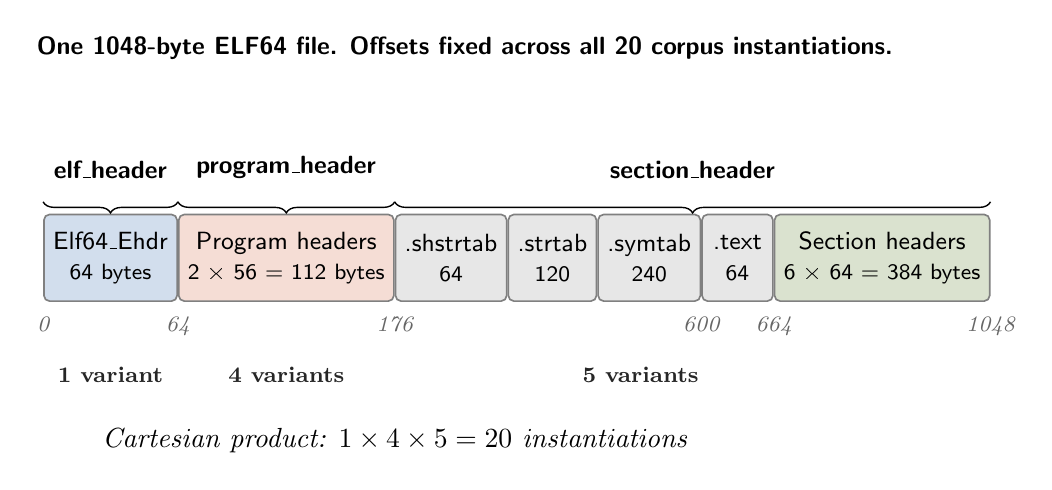
\begin{tikzpicture}[
  font=\sffamily\small,
  region/.style={draw=black!50, rounded corners=2pt, minimum height=1.1cm, align=center, line width=0.6pt},
  fixedlabel/.style={font=\footnotesize\itshape, text=black!60},
  varied/.style={font=\footnotesize\bfseries, text=black!85},
]

% Title row showing the byte offsets
\node[anchor=south] at (4.5,2.4) {\textbf{One 1048-byte ELF64 file. Offsets fixed across all 20 corpus instantiations.}};

% Linear ELF layout, drawn left-to-right
\node[region, fill=ehdrcolor!25, minimum width=1.4cm] (ehdr) at (0,0) {Elf64\_Ehdr\\\footnotesize 64 bytes};
\node[region, fill=phdrcolor!25, minimum width=1.8cm, right=0pt of ehdr] (phdr) {Program headers\\\footnotesize 2 × 56 = 112 bytes};
\node[region, fill=datcolor!25, minimum width=1.0cm, right=0pt of phdr] (shstr) {.shstrtab\\\footnotesize 64};
\node[region, fill=datcolor!25, minimum width=1.0cm, right=0pt of shstr] (strtab) {.strtab\\\footnotesize 120};
\node[region, fill=datcolor!25, minimum width=1.1cm, right=0pt of strtab] (symtab) {.symtab\\\footnotesize 240};
\node[region, fill=datcolor!25, minimum width=0.9cm, right=0pt of symtab] (text) {.text\\\footnotesize 64};
\node[region, fill=seccolor!25, minimum width=1.9cm, right=0pt of text] (shdrs) {Section headers\\\footnotesize 6 × 64 = 384 bytes};

% Byte offset markers
\node[fixedlabel, below=2pt of ehdr.south west] {0};
\node[fixedlabel, below=2pt of ehdr.south east] {64};
\node[fixedlabel, below=2pt of phdr.south east] {176};
\node[fixedlabel, below=2pt of symtab.south east] {600};
\node[fixedlabel, below=2pt of text.south east] {664};
\node[fixedlabel, below=2pt of shdrs.south east] {1048};

% Template-region braces above
\draw[decorate, decoration={brace, amplitude=4pt, mirror}, line width=0.5pt]
  ($(ehdr.north west)+(0,0.15)$) -- ($(ehdr.north east)+(0,0.15)$)
  node[midway, above=5pt] {\textbf{elf\_header}};
\draw[decorate, decoration={brace, amplitude=4pt, mirror}, line width=0.5pt]
  ($(phdr.north west)+(0,0.15)$) -- ($(phdr.north east)+(0,0.15)$)
  node[midway, above=5pt] {\textbf{program\_header}};
\draw[decorate, decoration={brace, amplitude=4pt, mirror}, line width=0.5pt]
  ($(shstr.north west)+(0,0.15)$) -- ($(shdrs.north east)+(0,0.15)$)
  node[midway, above=5pt] {\textbf{section\_header}};

% Variant counts under each child
\node[varied, below=20pt of ehdr] {1 variant};
\node[varied, below=20pt of phdr] {4 variants};
\node[varied, below=20pt of $(shstr.south east)!0.5!(shdrs.south west)$] {5 variants};

% Cartesian product line at bottom
\node[font=\itshape, below=42pt of phdr.south east] (cp) {Cartesian product: $1 \times 4 \times 5 = 20$ instantiations};

\end{tikzpicture}
\end{document}
